% !TEX root = ../swarthmore_talk.tex

% Odd Degree Galois
\begin{frame}[plain]
\ctext{Classification over Odd Degree Galois Fields}
\end{frame}



% Odd Degree Galois Classification
\begin{frame}[plain,c]
\begin{thm}[M.]
The set $\Phi_\Q^{\Gal,\text{odd}}(d^\infty)$ is finite, and if $E(K)_\tors \in \Phi_\Q^{\Gal,\text{odd}}(d^\infty)$, then $E(K)_\tors$ is precisely one of the following:
	\[
	\begin{cases}
	\Z/n\Z, & n= 1, 2, \ldots, 14, 18, 19, 21, 25, 27, 43, 67, 163 \text{ or} \\
	\Z/2\Z \oplus \Z/2n\Z, & n= 1, 2, 3, 4, 7.
	\end{cases}
	\]
Moreover, each such possibility occurs. 
\end{thm}
	\[
	\Phi_\Q^{\Gal,\text{odd}}(d^\infty):= \bigcup_{\substack{d \in \N \\ d \text{ odd}}} \Phi_\Q^{\Gal}(d)
	\]
\end{frame}



% Odd Degree Galois by Degree Table
\begin{frame}[plain,c]
        \begin{table}[!ht]
        \centering
        \resizebox{0.72\textwidth}{!}{%
        \begin{tabular}{>{\raggedright\arraybackslash}p{2.4cm}|%
           >{\centering\arraybackslash}p{5cm}||%
           >{\raggedright\arraybackslash}p{2.6cm}|%
           >{\centering\arraybackslash}p{5cm}%
          } \hline
        $F(d)^+$ & $\Phi_\Q^{\Gal}(d)$ & $F(d)^+$ & $\Phi_\Q^{\Gal}(d)$  \\ \hline
        & & & \\ %
        $(0,0,0^+,0^+)$ & $\Phi(1)$ & $(2,0,1^+,1^+)$ & $\Phi_\Q(3) \cup \{ \Z/19\Z, \Z/27\Z,$ $\Z/43\Z, \Z/67\Z \}$ \\
        & & & \\ %
        $(0,1,0^+,0^+)$ & $\Phi_\Q(5)$ & $(2,1^+,0,0)$ & $\Phi_\Q(3) \cup \Phi_\Q(5) \cup \{ \Z/19\Z, \Z/27\Z \}$ \\
        & & & \\ %
        $(1,0,0,0)$ & $\Phi_\Q(3)$ & $(2,1^+,0,1^+)$ & $\Phi_\Q(3) \cup \Phi_\Q(5) \cup \{ \Z/19\Z, \Z/27\Z, \Z/67\Z \}$ \\
        & & & \\ %
        $(1,0,0,1^+)$ & $\Phi_\Q(3) \cup \{ \Z/11\Z \}$ & $(2,1^+,1^+,0)$ & $\Phi_\Q(3) \cup \Phi_\Q(5) \cup \{ \Z/19\Z, \Z/27\Z, \Z/43\Z \}$ \\
        & & & \\ %
        $(1,0,1^+,0)$ & $\Phi_\Q(3) \cup \{ \Z/43\Z \}$ & $(2,1^+,1^+,1^+)$ & $\Phi_\Q(3) \cup \Phi_\Q(5) \cup \{ \Z/19\Z, \Z/27\Z, \Z/43\Z,$ $\Z/67\Z \}$ \\
        & & & \\ %
        $(1,0,1^+,1^+)$ & $\Phi_\Q(3) \cup \{ \Z/11\Z, \Z/43\Z \}$ & $(4^+,0,0,0)$ & $\Phi_\Q(3) \cup \{ \Z/19\Z, \Z/27\Z,$ $\Z/163\Z \}$ \\
        & & & \\ %
        $(1,1^+,0,0)$ & $\Phi_\Q(3) \cup \Phi_\Q(5)$ & $(4,0,0,1^+)$ & $\Phi_\Q(3) \cup \{ \Z/19\Z, \Z/27\Z,$ $\Z/67\Z, \Z/163\Z \}$ \\
        & & & \\ %
        $(1,1^+,0,1^+)$ & $\Phi_\Q(3) \cup \Phi_\Q(5) \cup \{ \Z/67\Z \}$ & $(4,0,1^+,0)$ & $\Phi_\Q(3) \cup \{ \Z/19\Z, \Z/27\Z,$ $\Z/47\Z, \Z/163\Z \}$ \\
        & & & \\ %
        $(1,1^+,1^+,0)$ & $\Phi_\Q(3) \cup \Phi_\Q(5) \cup \{ \Z/43\Z \}$ & $(4,0,1^+,1^+)$ & $\Phi_\Q(3) \cup \{ \Z/19\Z, \Z/27\Z,$ $\Z/43\Z, \Z/67\Z, \Z/163\Z \}$ \\
        & & & \\ %
        $(1,1^+,1^+,1^+)$ & $\Phi_\Q(3) \cup \Phi_\Q(5) \cup \{ \Z/43\Z,$ $\Z/67\Z \}$ & $(4,1^+,0,0)$ & $\Phi_\Q(3) \cup \Phi_\Q(5) \cup \{ \Z/19\Z, \Z/27\Z, \Z/163\Z \}$ \\
        & & & \\ %
        $(2,0,0,0)$ & $\Phi_\Q(3) \cup \{ \Z/19\Z, \Z/27\Z \}$ & $(4,1^+,0,1^+)$ & $\Phi_\Q(3) \cup \Phi_\Q(5) \cup \{ \Z/19\Z,$ $\Z/27\Z, \Z/67\Z, \Z/163\Z \}$ \\
        & & & \\ %
        $(2,0,0,1^+)$ & $\Phi_\Q(3) \cup \{ \Z/19\Z, \Z/27\Z,$ $\Z/67\Z \}$ & $(4,1^+,1^+,0)$ & $\Phi_\Q(3) \cup \Phi_\Q(5) \cup \{ \Z/19\Z,$ $\Z/27\Z, \Z/43\Z, \Z/163\Z \}$ \\
        & & & \\ %
        $(2,0,1^+,0)$ & $\Phi_\Q(3) \cup \{ \Z/19\Z, \Z/27\Z,$ $\Z/43\Z \}$ & $(4^+,1^+,1^+,1^+)$ & $\Phi_\Q(3) \cup \Phi(5) \cup \{ \Z/19\Z,$ $\Z/27\Z, \Z/43\Z, \Z/67\Z, \Z/163\Z \}$
        \end{tabular}%
        }
        \end{table}
\end{frame}















% Nonic Galois Field
\begin{frame}[plain]
\ctext{Classification over Nonic Galois Fields}
\end{frame}



% Quartic Galois Rational EC
\begin{frame}[plain]
\small
\begin{thm}[Chou, 2015]
Let $E/\Q$ be a rational elliptic curve, and let $K/\Q$ be a quartic Galois number field. Then the possible torsion subgroups $E(K)_\tors$ are precisely:
	\[
	\begin{cases}
	\Z/n\Z, & \text{with } n= 1, 2, \ldots, 10, 12, 13, 15, 16 \text{ or} \\
	\Z/2\Z \oplus \Z/2n\Z, & \text{with } n= 1, 2, \ldots, 6, 8 \text{ or} \\
	\Z/3\Z \oplus \Z/3n\Z, & \text{with } n= 1, 2 \text{ or} \\
	\Z/4\Z \oplus \Z/4n\Z, & \text{with } n= 1, 2 \text{ or} \\
	\Z/5\Z \oplus \Z/5\Z, & \text{or} \\
	\Z/6\Z \oplus \Z/6\Z.
	\end{cases}
	\]
\end{thm}
	\begin{figure}[!ht]
	\centering
	\captionsetup{labelformat=empty}
	\fbox{
\includegraphics[width=0.20\textwidth]{images/chou.jpg}}
	\caption{Michael Chou}
	\end{figure}
\end{frame}



% Outline
\begin{frame}[plain]
\frametitle{Outline of the Classification}
        \begin{enumerate}
        \item Determine the possible prime orders. \vfill
        \item Bound the $p$-Sylow Subgroups. \vfill
        \item Create a finite list of possibilities. \vfill
        \item Find examples and eliminate cases. \vfill
        \end{enumerate}
\vfill
\end{frame}



% Step 1. Determine the Possible Prime Orders
\begin{frame}[plain]
\vfill
\begin{center} {\bfseries \Large \textcolor{SwarthGarnet}{Step 1. Determine the Possible Prime Orders}} \end{center}
\vfill 
\end{frame}



% Lozano-Robledo S(d)
\begin{frame}[plain]
\begin{thm}[Lozano-Robledo, 2013]
Let $S_\Q(d)$ be the set of primes such that there exists an elliptic curve $E/\Q$ with a point of order $p$ defined in an extension $K/\Q$ of degree at most $d$. Then $S_\Q(9)= \{ 2, 3, 5, 7, 11, 13, 17, 19 \}$.
\end{thm}
	\begin{figure}[h]
	\centering
	\begin{subfigure}{\textwidth}
	\captionsetup{labelformat=empty}
	\centering
	\fbox{
\includegraphics[width=0.2\textwidth]{images/robledo.jpg}}
	\caption{\'Alvaro Lozano-Robledo}
	\end{subfigure}
	\end{figure}

\begin{rem}
Lozano-Robledo computes $S_\Q(d)$ for $1 \leq d \leq 21$ and gives a conjectural formula for $d \geq 1$, which is valid for $1 \leq d \leq 42$, which would follow from a positive answer to Serre's uniformity question. 
\end{rem}
\end{frame}



% Gonzalez-Jimenez, Najman R(d)
\begin{frame}[plain]
\begin{prop}[Gonz\'alez-Jim\'enez, Najman, 2016] \hfill
	\begin{enumerate}[(i)]
	\item $11 \in R_\Q(d)$ if and only if $5 \mid d$.
	\item $17 \in R_\Q(d)$ if and only if $8 \mid d$.
	\end{enumerate}
\end{prop}
	\begin{figure}[h]
	\centering
	\begin{subfigure}{0.35\textwidth}
	\captionsetup{labelformat=empty}
	\centering
	\fbox{
\includegraphics[width=0.65\textwidth]{images/jimenez.png}}
	\caption{Enrique Gonz\'alez-Jim\'enez}
	\end{subfigure}
	%
	\begin{subfigure}{0.3\textwidth}
	\captionsetup{labelformat=empty}
	\centering
	\fbox{
\includegraphics[width=0.70\textwidth]{images/najman2.png}}
	\caption{Filip Najman}
	\end{subfigure}
	\end{figure}
\end{frame}



% Prime Possible
\begin{frame}[plain]
\begin{prop}
Let $E/\Q$ be a rational elliptic curve, and let $K/\Q$ be a nonic Galois field. If $P \in E(K)$ is a point of prime order $p$, then $p \in \{ 2, 3, 5, 7, 13,$ $19 \}$.
\end{prop}
\end{frame}



% Step 2. Bound the Size of the Sylow Subgroups
\begin{frame}[plain]
\vfill
\begin{center} {\bfseries \Large \textcolor{SwarthGarnet}{Step 2. Bound the Size of the Sylow Subgroups}} \end{center}
\vfill 
\end{frame}



% Full 2-Torsion, Lozano-Robledo
\begin{frame}[plain]
\begin{thm}[Gonz\'alez-Jim\'enez, Lozano-Robledo]
Let $E/\Q$ be an elliptic curve without CM. Let $1 \leq s \leq N$ be fixed integers, and let $T \subseteq E[2^N]$ be a subgroup isomorphic to $\Z/2^s/Z \oplus \Z/2^N \Z$. Then $[\Q(T) \colon \Q]$ is divisible by 2 if $s=N=2$, and otherwise by $2^{2N+2s-8}$ if $N \geq 3$, unless $s \geq 4$ and $j(E)$ is one of the two values:
	\[
	- \dfrac{3 \cdot 18249920^3}{17^{16}}\; \text{ or } - \dfrac{7 \cdot 1723187806080^3}{79^{16}}
	\]
in which case $[\Q(T) \colon \Q]$ is divisible by $3 \cdot 2^{2N+2s-9}$. Moreover, this is best possible in that there are one-parameter families $E_{s,N}(t)$ of elliptic curves over $\Q$ such that for each $s, N \geq 0$ and each $t \in \Q$, and subgroups $T_{s,N} \in E_{s,N}(t)(\ov{\Q})$ isomorphic to $\Z/2^s\Z \oplus \Z/2^N\Z$ such that $[\Q(T_{s,N}) \colon \Q]$ is equal to the bound given above. 
\end{thm}
\end{frame}



% 2-Sylow Bound
\begin{frame}[plain]
\begin{lem}[2-Sylow Bound]
Let $E/\Q$ be a rational elliptic curve, and let $K/\Q$ be a nonic Galois field. Then $E(K)[2^\infty] \subseteq \Z/2\Z \oplus \Z/8\Z$.
\end{lem}
\end{frame}



% Full p-Torsion & Weil-Pairing
\begin{frame}[plain]
\footnotesize
\phantom{.} \vfill
\begin{lem}[Odd Torsion]
Let $K/\Q$ be an odd degree number field, and let $E/\Q$ be a rational elliptic curve. Then $E(K)_\tors$ does not contain full $p$-torsion for all odd primes.
\end{lem}

\pf By the existence of the Weil-pairing, if $E(K)$ contains full $p$-torsion, then $\Q(\zeta_p) \subseteq K$. But for $p > 2$, $[\Q(\zeta_p) \colon \Q]= \phi(p)$ is even, a contradiction. \hfill \qed \vfill
\end{frame}



% Full p-Torsion & Weil-Pairing 2
\begin{frame}[plain]
\footnotesize
\begin{lem}[Galois Isogeny]
Let $K/\Q$ be a Galois extension, and let $E/\Q$ be a rational elliptic curve. If $E(K)[n] \cong \Z/n\Z$, then $E$ has a rational $n$-isogeny. 
\end{lem} \vfill

\begin{lem}[Galois Isogeny]
Let $E/\Q$ be a rational elliptic curve, and let $K/\Q$ be a Galois extension. If $E(K)_\tors \cong \Z/m\Z \oplus \Z/mn\Z$, then $E$ has a rational $n$-isogeny. 
\end{lem} \vfill

\begin{thm}[Fricke, Kenku, Klein, Kubert, Ligozat, Mazur, Ogg, et al.]
Let $N \geq 2$ be such that $X_0(N)$ has a non-cuspidal $\Q$-rational point. Then
	\begin{enumerate}[(i)]
	\item $N \leq 10$ or $N=$ 12, 13, 16, 18, or 25. In this case, $X_0(N)$ is a curve of genus 0, and the $\Q$ rational points on $X_0(N)$ form an infinite 1-parameter family, or
	\item $N=$ 11, 14, 15, 17, 19, 21, or 27, i.e. $X_0(N)$ is a rational elliptic curve (in each case $X_0(N)(\Q)$ is finite, or
	\item $N=$ 37, 43, 67, or 163. In this case, $X_0(N)$ is a curve of genus $\geq 2$ and by Faltings' Theorem has only finitely many $\Q$-rational points. 
	\end{enumerate}
In particular, a rational elliptic curve may only have a rational cyclic $n$-isogeny for $n \leq 19$ or $n \in \{ 21, 25, 27, 37, 43, 67,163\}$. Furthermore, if $E$ does not have CM, then $n \leq 18$ or $n \in \{ 21, 25, 37 \}$.
\end{thm}
\end{frame}



% Sylow Bounds
\begin{frame}[plain]
\footnotesize
\begin{lem}[$p$-Sylow bounds]
Let $E/\Q$ be a rational elliptic curve, and let $K/\Q$ be a nonic Galois field. Then
	\[
	\begin{aligned}
	E(K)[2^\infty]&\subseteq \Z/2\Z \oplus \Z/8\Z \\
	E(K)[3^\infty]&\subseteq \Z/27\Z \\
	E(K)[5^\infty]&\subseteq \Z/25\Z \\
	E(K)[7^\infty]&\subseteq \Z/7\Z \\
	E(K)[13^\infty]&\subseteq \Z/13\Z \\
	E(K)[19^\infty]&\subseteq \Z/19\Z
	\end{aligned}
	\]
\end{lem}
\end{frame}



% Step 3. Create a Finite List of Possibilities
\begin{frame}[plain]
\vfill
\begin{center} {\bfseries \Large \textcolor{SwarthGarnet}{Step 3. Create a Finite List of Possibilities}} \end{center}
\vfill 
\end{frame}



% Finite List
\begin{frame}[plain]
\footnotesize
\begin{lem}
Let $E/\Q$ be a rational elliptic curve, and let $K/\Q$ be a nonic Galois field. Then $E(K)_\tors$ is isomorphic to one of the following (although not all cases need occur):
	\[
	\begin{cases}
	\Z/n\Z, & n= 1, 2, \ldots, 10, 12, 13, 14, 15, 18, 19, 21, 25, 27 \\
	\Z/2\Z \oplus \Z/2n\Z, & n= 1, 2, \ldots, 7, 9, 10, 12, 13, 14, 15, 18, 19, 21, 25, 27
	\end{cases}
	\]
\end{lem} 
\end{frame}



% Step 4. Find Examples \& Eliminate Cases
\begin{frame}[plain]
\vfill
\begin{center} {\bfseries \Large \textcolor{SwarthGarnet}{Step 4. Find Examples \& Eliminate Cases}} \end{center}
\vfill 
\end{frame}



% Upstairs/Downstairs Games
\begin{frame}[plain] \frametitle{}
	\vspace{1cm} \vfill 
	
	\begin{center}
	{\color{SwarthGarnet}\Large\bfseries Upstairs/Downstairs Games}
	\end{center}
	
	\begin{figure}[h,t]
	\centering
	\begin{subfigure}{\textwidth}
	\captionsetup{labelformat=empty}
	\centering
	\fbox{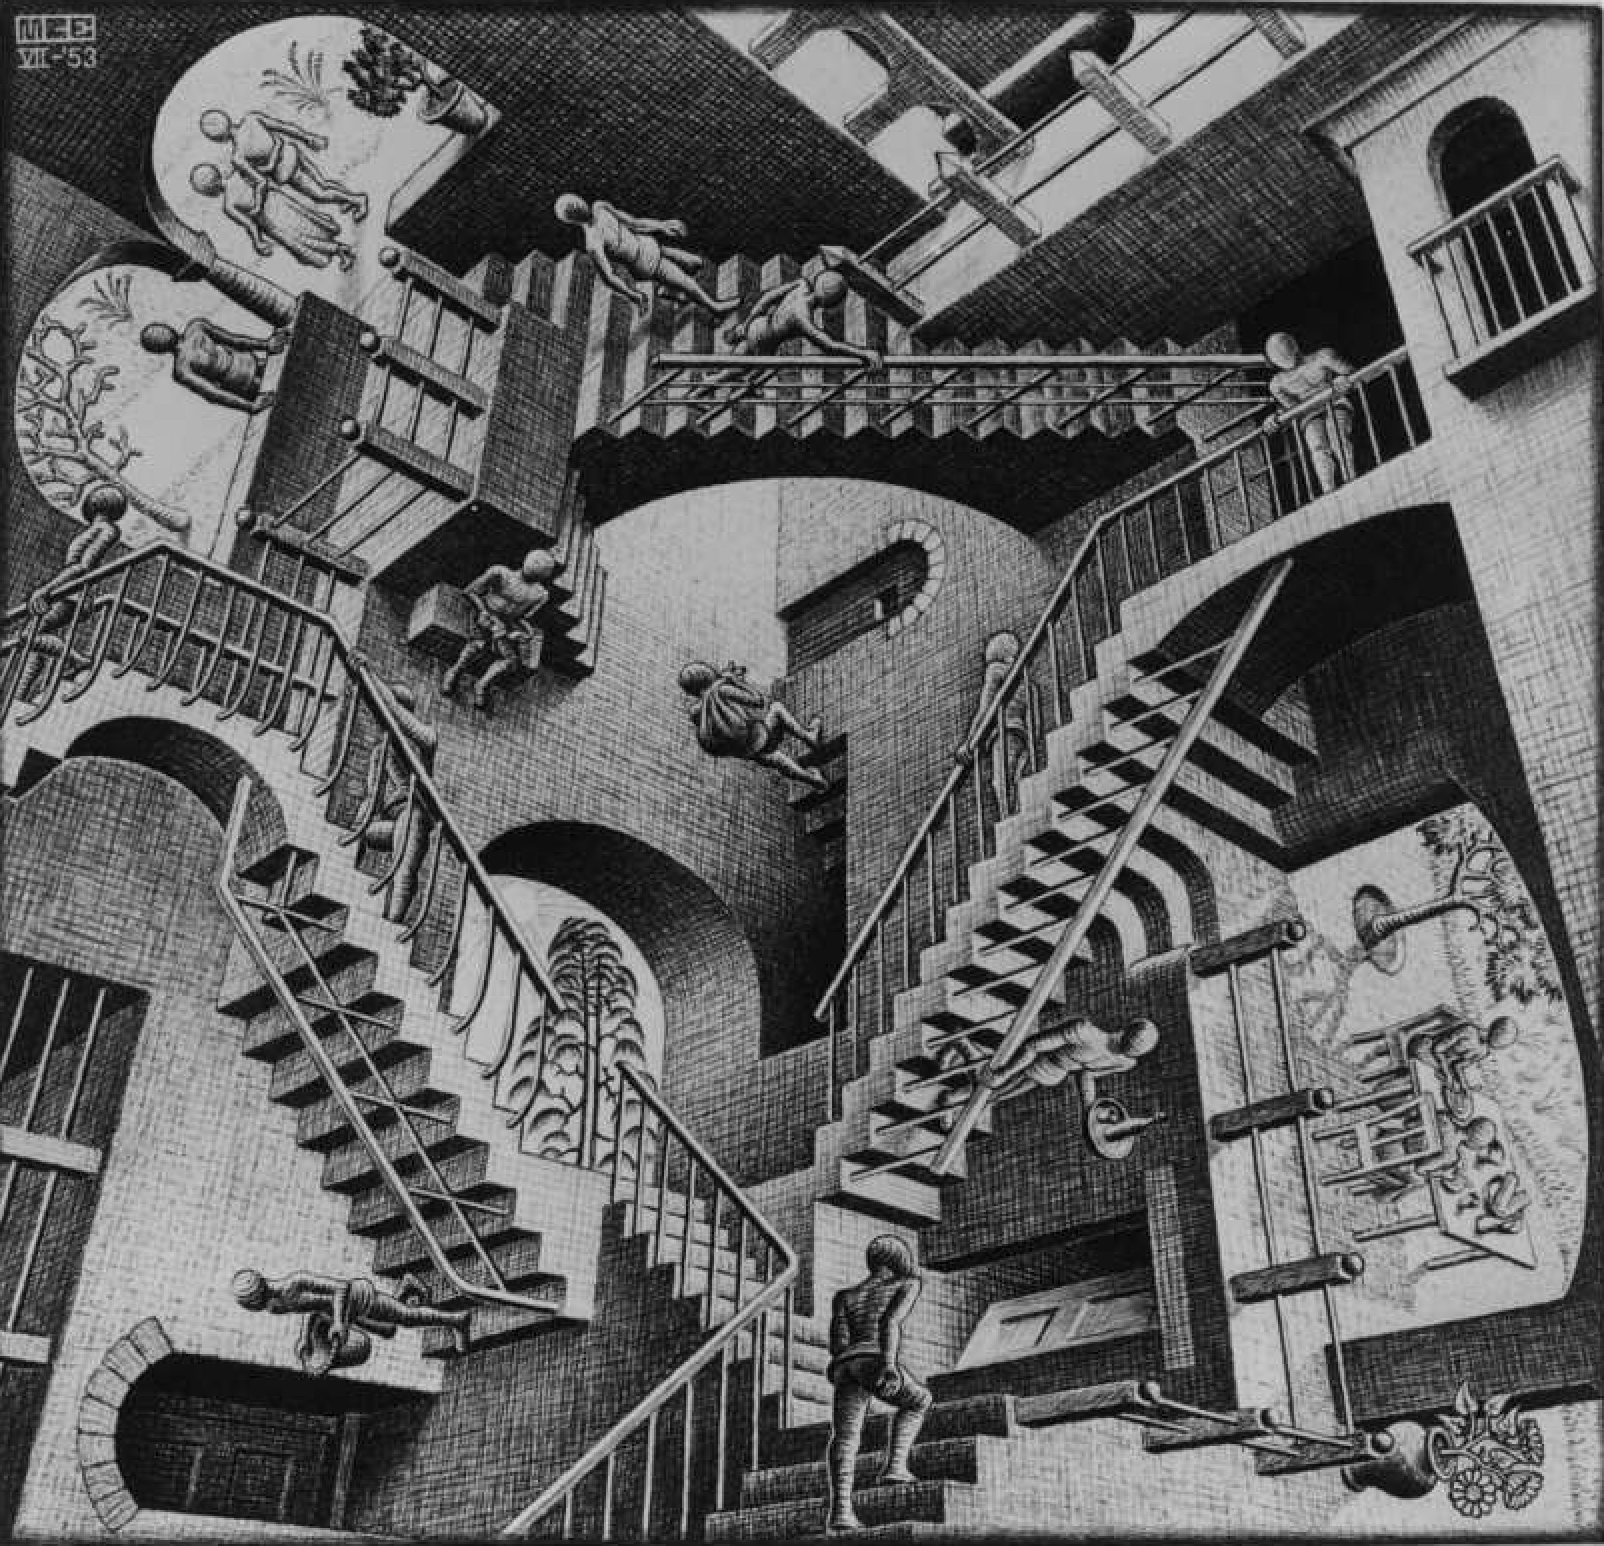
\includegraphics[width=0.6\textwidth]{images/escher.png}}
	\caption{M.C. Escher's Relativity}
	\end{subfigure}
	\end{figure}
\end{frame}



% Base Extension
\begin{frame}[plain]
\begin{prop}
Let $E/\Q$ be a rational elliptic curve, and let $F/\Q$ be a cubic Galois field. Then there exists a nonic Galois field $K$ such that $E(K)_\tors \cong E(F)_\tors$.
\end{prop}

\pf 
\begin{itemize}
\item If $F_1, F_2$ are distinct cubic Galois fields, then $F_1F_2$ is a nonic Galois extension. It suffices to prove there are infinitely many distinct cubic Galois fields. 
\item For a chosen integer $k$, define $a:= k^2 + k + 7$.
\item The field $K_a:= \Q(x^3 - ax + a)$ is a cubic Galois field. For each distinct $a$, the fields $K_a$ are distinct. \hfill\qed
\end{itemize}

\begin{cor}
$\Phi_\Q^{\Gal}(3) \subseteq \Phi_\Q^{\Gal}(9)$
\end{cor}
\end{frame}



% Examples of Torsion Subgroups
\begin{frame}[plain]
	\begin{table}[!ht]
	\centering
	\caption{Examples of torsion subgroups $\Phi_\Q(3) \setminus \Phi(1)$.\label{tab:3qsm1}}
	\begin{tabular}{ccc} \hline
	Torsion Subgroup & Elliptic Curve & Galois Cubic Field \\ \hline
	$\Z/13\Z$ & \ofsbo{} & \qzetasp{} \\
	$\Z/14\Z$ & \fnat{} & \qzetasp{} \\
	$\Z/18\Z$ & \ofaf{} & \qzetasp{} \\
	$\Z/21\Z$ & \ostbo{} & \qzetanp{} \\
	$\Z/2\Z \times \Z/14\Z$ & \onttco{} & \ttnsoo{}
	\end{tabular}
	\end{table}

        \begin{table}[!ht]
        \centering
        \caption{Examples of $E(K)$ with 19 and 27-torsion over nonic fields.\label{tab:1927tor}}
        \begin{tabular}{cccc} \hline
        $E(K)_\tors$ & $E(\Q)_\tors$ &  $E$ & $K$ \\ \hline
        $\Z/19\Z$ & $\{ \O \}$ & \tsoao{} & \qzetantp{} \\ 
        $\Z/27\Z$ & $\Z/3\Z$ & \tsaf{} & \qzetatsp{}
        \end{tabular}
        \end{table}
\end{frame}



% Remaining Groups
\begin{frame}[plain]
This leaves the following list of torsion subgroups whose existence or non-existence we have yet to prove. \pspace
	\[
	\begin{cases}
	\Z/n\Z, & n= 15, 25 \\
	\Z/2\Z \oplus \Z/2n\Z, & n= 5, 6, 9, 10, 12, 13, 14, 15, 18, 19, 21, 25, 27
	\end{cases}
	\]
\end{frame}



% Najman Growth Lemmas
\begin{frame}[plain]
\begin{lem}[Najman, 2015]
Let $p, q$ be distinct odd primes, $F_2/F_1$ a Galois extension of number fields such that $\Gal(F_2/F_1) \simeq \Z/q\Z$ and $E/F_1$ an elliptic curve with no $p$-torsion over $F_1$. Then if $q$ does not divide $p-1$ and $\Q(\zeta_p) \not\subset F_2$, then $E(F_2)[p]=0$. 
\end{lem}

\begin{lem}[Najman, 2015]
Let $p$ be an odd prime number, $q$ a prime not dividing $p$, $F_2/F_1$ a Galois extension of number fields such that $\Gal(F_2/F_1) \simeq \Z/q\Z$, $E/F_1$ an elliptic curve, and suppose $E(F_1) \supset \Z/p\Z$, $E(F_1) \not\supset \Z/p^2\Z$, and $\zeta_p \notin F_2$. Then $E(F_2) \not\supset \Z/p^2\Z$.
\end{lem} 
\end{frame}



% Field of Definition Degree
\begin{frame}[plain]
\begin{prop}
Let $E/\Q$ be a rational elliptic curve, and let $K/\Q$ be a nonic Galois field. Suppose $P \in E(K)_\tors$ is a point of order $p$. Then
        \begin{enumerate}[(i)]
        \item if $p \in \{ 3, 5 \}$, then $P$ is defined over $\Q$, i.e. $P \in E(\Q)[p]$.
        \item if $p= 13$, then there is a cubic field $F \subseteq K$ with $P \in E(F)[p]$. 
        \item if $p \in \{ 2, 7 \}$, then $P$ is defined over $\Q$, i.e. $P \in E(\Q)[p]$, or there is a cubic field $F \subseteq K$ with $P \in E(F)[p]$. 
        \end{enumerate}
\end{prop}
\end{frame}



% Z/2Z x Z/10Z
\begin{frame}[plain]
\footnotesize
\begin{lem}
Let $E/\Q$ be a rational elliptic curve, and let $K/\Q$ be a nonic Galois field. Then $E(K)_\tors$ does not contain $\Z/2\Z \oplus \Z/10\Z$.
\end{lem} \pspace

\pf
\begin{itemize}
\item By our previous result, we know that $E(K)[5^\infty]= E(\Q)[5^\infty] \cong \Z/5\Z$. 
\item Choosing a model $E: y^2= x^3 + Ax + B$, we know the $x$-coordinates of points of order 2 correspond to roots of $x^3 + Ax + B$. 
\item As $E(K)_\tors \supseteq \Z/2\Z \oplus \Z/2\Z$, $K$ contains a splitting field for $x^3 + Ax + B$, which has degree 1, 3, or 6. 
\item Degree 6 is not possible as $K/\Q$ has odd degree. Then $\Q(E(K)[2^\infty])$ is defined over at most a cubic field. 
\item But then either $E(\Q)_\tors \cong \Z/2\Z \oplus \Z/10\Z$ or there is a cubic field, $F$, with $E(F)_\tors \cong \Z/2\Z \oplus \Z/10\Z$, contradicting the classification of either $\Phi(1)$ or $\Phi_\Q(3)$. \hfill\qed
\end{itemize}
\end{frame}



% Nonic Galois Result
\begin{frame}[plain]
\begin{thm}[M.]
Let $E/\Q$ be a rational elliptic curve, and let $K/\Q$ be a nonic Galois field. Then $E(K)_\tors$ is isomorphic to precisely one of the following:
	\[
	\begin{cases}
	\Z/n\Z, & n= 1, 2, \ldots, 10, 12, 13, 14, 18, 19, 21, 27 \\
	\Z/2\Z \oplus \Z/2n\Z, & n= 1, 2, 3, 4, 7
	\end{cases}
	\]
\end{thm}
\end{frame}



% Nonic Galois Examples
\begin{frame}[plain]
	\begin{table}[!ht]
	\centering
	\caption{Examples of each possible $E(K)_\tors$ in $\Phi_\Q^{\Gal}(9)$.}
	\resizebox{!}{0.36\textwidth}{%
	\begin{tabular}{cccc} \hline
	 $E(K)_\tors$ & Cremona Label & $E(\Q)_\tors$ & $K$ \\ \hline
	$\{ \O \}$ & \ooat{} & $\{ \O \}$ & \qzetantp{} \\
	$\Z/2\Z$ & \ffafiv{} & $\Z/2\Z$ & \qzetantp{} \\
	$\Z/3\Z$ & \onao{} & $\Z/3\Z$ & \qzetantp{} \\
	$\Z/4\Z$ & \ofas{} & $\Z/4\Z$ & \qzetantp{} \\
	$\Z/5\Z$ & \ooao{} & $\Z/5\Z$ & \qzetantp{} \\
	$\Z/6\Z$ & \ofat{} & $\Z/6\Z$ & \qzetantp{} \\
	$\Z/7\Z$ & \tsbo{} & $\Z/7\Z$ & \qzetantp{} \\
	$\Z/8\Z$ & \ffafo{} & $\Z/8\Z$ & \qzetantp{} \\
	$\Z/9\Z$ & \ffbt{} & $\Z/9\Z$ & \qzetantp{} \\
	$\Z/10\Z$ & \ssco{} & $\Z/10\Z$ & \qzetantp{} \\
	$\Z/12\Z$ & \nzct{} & $\Z/12\Z$ & \qzetantp{} \\
	$\Z/13\Z$ & \ofsbo{} & $\{ \O \}$ & \qzetantp{} \\
	$\Z/14\Z$ & \fnaf{} & $\Z/2\Z$ & \qzetantp{} \\
	$\Z/18\Z$ & \tszsozot{} & $\Z/6\Z$ & \nnezsb{} \\
	$\Z/19\Z$ & \tsoao{} & $\{ \O \}$ & \qzetantp{} \\
	$\Z/21\Z$ & \ostbo{} & $\Z/3\Z$ & \nnstfttf{} \\
	$\Z/27\Z$ & \tsaf{} & $\Z/3\Z$ & \qzetatsp{} \\
	$\Z/2\Z \oplus \Z/2\Z$ & \ffat{} & $\Z/2\Z \oplus \Z/2\Z$ & \qzetantp{} \\
	$\Z/2\Z \oplus \Z/4\Z$ & \ffao{} & $\Z/2\Z \oplus \Z/4\Z$ & \qzetantp{} \\
	$\Z/2\Z \oplus \Z/6\Z$ & \tzat{} & $\Z/2\Z \oplus \Z/6\Z$ & \qzetantp{} \\
	$\Z/2\Z \oplus \Z/8\Z$ & \tozet{} & $\Z/2\Z \oplus \Z/8\Z$ & \qzetantp{} \\
	$\Z/2\Z \oplus \Z/14\Z$ & \onttco{} & $\{ \O \}$ & \nnstfttfz{} \\
	\end{tabular}
	}
	\end{table}
\end{frame}



% General Nonic Conjecture
\begin{frame}[plain]
\footnotesize
\begin{conj}
Let $E/\Q$ be a rational elliptic curve, and let $K/\Q$ be a nonic field. Then $E(K)_\tors$ is isomorphic to precisely one of the following:
	\[
	\begin{cases}
	\Z/n\Z, & \text{with } n= 1, 2, \ldots, 10, 12, 13, 14, 18, 19, 21, 26, 27, 28, 36, 42 \\
	\Z/2\Z \oplus \Z/2n\Z, & \text{with } n= 1, 2, 3, 4, 7, 9
	\end{cases}
	\]
Moreover, each such possibility occurs.
\end{conj}
\end{frame}



% Torsion Growth Result
\begin{frame}[plain]
\ctext{Torsion Growth over Nonic Galois Fields}
\end{frame}



% Torsion Growth Result 2
\begin{frame}[plain]
\begin{table}[]
\centering
\resizebox{!}{0.33\textwidth}{%
\begin{tabular}{|l|c|c|c|c|c|c|c|c|c|c|c|c|c|c|c|} \hline
\diagbox[width=6.8em]{$E(K)_\tors$}{$E(\Q)_\tors$}
 & $\mathcal{C}_1$ & $\mathcal{C}_2$ & $\mathcal{C}_3$ & $\mathcal{C}_4$ & $\mathcal{C}_5$ & $\mathcal{C}_6$ & $\mathcal{C}_7$ & $\mathcal{C}_8$ & $\mathcal{C}_9$ & $\mathcal{C}_{10}$ & $\mathcal{C}_{12}$ & $\mathcal{C}_2 \times \mathcal{C}_2$ & $\mathcal{C}_2 \times \mathcal{C}_4$ & $\mathcal{C}_2 \times \mathcal{C}_6$ & $\mathcal{C}_2 \times \mathcal{C}_8$ \\ \hline
$\mathcal{C}_1$ & \cmark & \cellcolor[HTML]{000000} & \cellcolor[HTML]{000000} & \cellcolor[HTML]{000000} & \cellcolor[HTML]{000000} & \cellcolor[HTML]{000000} & \cellcolor[HTML]{000000} & \cellcolor[HTML]{000000} & \cellcolor[HTML]{000000} & \cellcolor[HTML]{000000} & \cellcolor[HTML]{000000} & \cellcolor[HTML]{000000} & \cellcolor[HTML]{000000} & \cellcolor[HTML]{000000} & \cellcolor[HTML]{000000} \\ \hline
$\mathcal{C}_2$ &  & \cmark & \cellcolor[HTML]{000000}{\color[HTML]{000000} } & \cellcolor[HTML]{000000} & \cellcolor[HTML]{000000} & \cellcolor[HTML]{000000} & \cellcolor[HTML]{000000} & \cellcolor[HTML]{000000} & \cellcolor[HTML]{000000} & \cellcolor[HTML]{000000} & \cellcolor[HTML]{000000} & \cellcolor[HTML]{000000} & \cellcolor[HTML]{000000} & \cellcolor[HTML]{000000} & \cellcolor[HTML]{000000} \\ \hline
$\mathcal{C}_3$ &  &  & \cmark & \cellcolor[HTML]{000000} & \cellcolor[HTML]{000000} & \cellcolor[HTML]{000000} & \cellcolor[HTML]{000000} & \cellcolor[HTML]{000000} & \cellcolor[HTML]{000000} & \cellcolor[HTML]{000000} & \cellcolor[HTML]{000000} & \cellcolor[HTML]{000000} & \cellcolor[HTML]{000000} & \cellcolor[HTML]{000000} & \cellcolor[HTML]{000000} \\ \hline
$\mathcal{C}_4$ &  &  &  & \cmark & \cellcolor[HTML]{000000} & \cellcolor[HTML]{000000} & \cellcolor[HTML]{000000} & \cellcolor[HTML]{000000} & \cellcolor[HTML]{000000} & \cellcolor[HTML]{000000} & \cellcolor[HTML]{000000} & \cellcolor[HTML]{000000} & \cellcolor[HTML]{000000} & \cellcolor[HTML]{000000} & \cellcolor[HTML]{000000} \\ \hline
$\mathcal{C}_5$ &  &  &  &  & \cmark & \cellcolor[HTML]{000000} & \cellcolor[HTML]{000000} & \cellcolor[HTML]{000000} & \cellcolor[HTML]{000000} & \cellcolor[HTML]{000000} & \cellcolor[HTML]{000000} & \cellcolor[HTML]{000000} & \cellcolor[HTML]{000000} & \cellcolor[HTML]{000000} & \cellcolor[HTML]{000000} \\ \hline
$\mathcal{C}_6$ &  &  &  &  &  & \cmark & \cellcolor[HTML]{000000} & \cellcolor[HTML]{000000} & \cellcolor[HTML]{000000} & \cellcolor[HTML]{000000} & \cellcolor[HTML]{000000} & \cellcolor[HTML]{000000} & \cellcolor[HTML]{000000} & \cellcolor[HTML]{000000} & \cellcolor[HTML]{000000} \\ \hline
$\mathcal{C}_7$ & \cmark &  &  &  &  &  & \cmark & \cellcolor[HTML]{000000} & \cellcolor[HTML]{000000} & \cellcolor[HTML]{000000} & \cellcolor[HTML]{000000} & \cellcolor[HTML]{000000} & \cellcolor[HTML]{000000} & \cellcolor[HTML]{000000} & \cellcolor[HTML]{000000} \\ \hline
$\mathcal{C}_8$ &  &  &  &  &  &  &  & \cmark & \cellcolor[HTML]{000000} & \cellcolor[HTML]{000000} & \cellcolor[HTML]{000000} & \cellcolor[HTML]{000000} & \cellcolor[HTML]{000000} & \cellcolor[HTML]{000000} & \cellcolor[HTML]{000000} \\ \hline
$\mathcal{C}_9$ &  &  & \cmark &  &  &  &  &  & \cmark & \cellcolor[HTML]{000000} & \cellcolor[HTML]{000000} & \cellcolor[HTML]{000000} & \cellcolor[HTML]{000000} & \cellcolor[HTML]{000000} & \cellcolor[HTML]{000000} \\ \hline
$\mathcal{C}_{10}$ &  &  &  &  &  &  &  &  &  & \cmark & \cellcolor[HTML]{000000} & \cellcolor[HTML]{000000} & \cellcolor[HTML]{000000} & \cellcolor[HTML]{000000} & \cellcolor[HTML]{000000} \\ \hline
$\mathcal{C}_{12}$ &  &  &  &  &  &  &  &  &  &  & \cmark & \cellcolor[HTML]{000000} & \cellcolor[HTML]{000000} & \cellcolor[HTML]{000000} & \cellcolor[HTML]{000000} \\ \hline
$\mathcal{C}_{13}$ & \cmark &  &  &  &  &  &  &  &  &  &  & \cellcolor[HTML]{000000} & \cellcolor[HTML]{000000} & \cellcolor[HTML]{000000} & \cellcolor[HTML]{000000} \\ \hline
$\mathcal{C}_{14}$ &  & \cmark &  &  &  &  &  &  &  &  &  & \cellcolor[HTML]{000000} & \cellcolor[HTML]{000000} & \cellcolor[HTML]{000000} & \cellcolor[HTML]{000000} \\ \hline
$\mathcal{C}_{18}$ &  &  &  &  &  & \cmark &  &  &  &  &  & \cellcolor[HTML]{000000} & \cellcolor[HTML]{000000} & \cellcolor[HTML]{000000} & \cellcolor[HTML]{000000} \\ \hline
$\mathcal{C}_{19}$ & \cmark &  &  &  &  &  &  &  &  &  &  & \cellcolor[HTML]{000000} & \cellcolor[HTML]{000000} & \cellcolor[HTML]{000000} & \cellcolor[HTML]{000000} \\ \hline
$\mathcal{C}_{21}$ &  &  & \cmark &  &  &  &  &  &  &  &  & \cellcolor[HTML]{000000} & \cellcolor[HTML]{000000} & \cellcolor[HTML]{000000} & \cellcolor[HTML]{000000} \\ \hline
$\mathcal{C}_{27}$ &  &  & \cmark &  &  &  &  &  &  &  &  & \cellcolor[HTML]{000000} & \cellcolor[HTML]{000000} & \cellcolor[HTML]{000000} & \cellcolor[HTML]{000000} \\ \hline
$\mathcal{C}_2 \times \mathcal{C}_2$ & \cmark &  &  &  &  &  &  &  &  &  &  & \cmark & \cellcolor[HTML]{000000} & \cellcolor[HTML]{000000} & \cellcolor[HTML]{000000} \\ \hline
$\mathcal{C}_2 \times \mathcal{C}_4$ &  &  &  &  &  &  &  &  &  &  &  &  & \cmark & \cellcolor[HTML]{000000} & \cellcolor[HTML]{000000} \\ \hline
$\mathcal{C}_2 \times \mathcal{C}_6$ &  &  & \cmark &  &  &  &  &  &  &  &  &  &  & \cmark & \cellcolor[HTML]{000000}{\color[HTML]{000000} } \\ \hline
$\mathcal{C}_2 \times \mathcal{C}_8$ &  &  &  &  &  &  &  &  &  &  &  &  &  &  & \cmark \\ \hline
$\mathcal{C}_2 \times \mathcal{C}_{14}$ & \cmark &  &  &  &  &  &  &  &  &  &  &  &  &  &  \\ \hline
\end{tabular}
}
\end{table}
\end{frame}



% Bicyclic
\begin{frame}[plain]
\ctext{Bicyclic Nonic Galois Fields}
\end{frame}



% Bicyclic Classification
\begin{frame}[plain]
\begin{thm}[M.]
Let $E/\Q$ be a rational elliptic curve, and let $K/\Q$ be a nonic bicyclic Galois field, i.e. a nonic field with $\Gal(K/\Q) \cong \Z/3\Z \oplus \Z/3\Z$. Then $E(K)_\tors$ is precisely one of the following:
	\[
	\begin{cases}
	\Z/n\Z, & n= 1, 2, \ldots, 10, 12, 13, 14, 18, 21 \\
	\Z/2\Z \oplus \Z/2n\Z, & n= 1, 2, 3, 4, 7
	\end{cases}
	\]
\end{thm}
\end{frame}



% Bicyclic Examples
\begin{frame}[plain]
	\begin{table}[!ht] 
	\centering
	\caption{Examples of torsion subgroups $E(K)_\tors$ in $\Phi_\Q^{\cC_3 \times \cC_3}(9)$.}
	\resizebox{!}{0.36\textwidth}{%
	\begin{tabular}{cccc} \hline
	 $E(K)_\tors$ & Cremona Label & $E(\Q)_\tors$ & $K$ \\ \hline
	$\{ \O \}$ & \ooat{} & $\{ \O \}$ & \nnstfttf{} \\
	$\Z/2\Z$ & \ffafiv{} & $\Z/2\Z$ & \nnstfttf{} \\
	$\Z/3\Z$ & \onao{} & $\Z/3\Z$ & \nnstfttf{} \\
	$\Z/4\Z$ & \ofas{} & $\Z/4\Z$ & \nnstfttf{} \\
	$\Z/5\Z$ & \ooao{} & $\Z/5\Z$ & \nnstfttf{} \\
	$\Z/6\Z$ & \ofat{} & $\Z/6\Z$ & \nnstfttf{} \\
	$\Z/7\Z$ & \tsbo{} & $\Z/7\Z$ & \nnstfttf{} \\
	$\Z/8\Z$ & \ffaf{} & $\Z/8\Z$ & \nnstfttf{} \\
	$\Z/9\Z$ & \ffbt{} & $\Z/9\Z$ & \nnstfttf{} \\
	$\Z/10\Z$ & \ssco{} & $\Z/10\Z$ & \nnstfttf{} \\
	$\Z/12\Z$ & \nzct{} & $\Z/12\Z$ & \nnstfttf{} \\
	$\Z/13\Z$ & \ofsbo{} & $\{ \O \}$ & \nnstfttf{} \\
	$\Z/14\Z$ & \fnaf{} & $\Z/2\Z$ & \nnstfttf{} \\
	$\Z/18\Z$ & \ofaf{} & $\Z/6\Z$ & \nnstfttf{} \\
	$\Z/21\Z$ & \ostbo{} & $\Z/3\Z$ & \qzetatsp{} \\
	$\Z/2\Z \oplus \Z/2\Z$ & \ffat{} & $\Z/2\Z \oplus \Z/2\Z$ & \nnstfttf{} \\
	$\Z/2\Z \oplus \Z/4\Z$ & \ffao{} & $\Z/2\Z \oplus \Z/4\Z$ & \nnstfttf{} \\
	$\Z/2\Z \oplus \Z/6\Z$ & \tzat{} & $\Z/2\Z \oplus \Z/6\Z$ & \nnstfttf{} \\
	$\Z/2\Z \oplus \Z/8\Z$ & \tozet{} & $\Z/2\Z \oplus \Z/8\Z$ & \nnstfttf{} \\
	$\Z/2\Z \oplus \Z/14\Z$ & \onttco{} & $\{ \O \}$ & \nnstfttfz{} \\
	\end{tabular}
	}
	\end{table}
\end{frame}



% Cyclic Nonic 
\begin{frame}[plain]
\ctext{Cyclic Nonic Galois Fields}
\end{frame}



% Cyclic Nonic Classification
\begin{frame}[plain]
\begin{thm}[M.]
Let $E/\Q$ be a rational elliptic curve, and let $K/\Q$ be a nonic cyclic Galois field, i.e. a nonic field with $\Gal(K/\Q) \cong \Z/9\Z$. Then $E(K)_\tors$ is precisely one of the following:
	\[
	\begin{cases}
	\Z/n\Z, & n= 1, 2, \ldots, 10, 12, 13, 14, 21 \\
	\Z/2\Z \oplus \Z/2n\Z, & n= 1, 2, 3, 4
	\end{cases}
	\]
\end{thm}
\end{frame}



% Cyclic Nonic Examples
\begin{frame}[plain]
	\begin{table}[!ht] 
	\centering
	\caption{Examples of torsion subgroups $E(K)_\tors$ in $\Phi_\Q^{\cC_9}(9)$.}
	\resizebox{!}{0.36\textwidth}{%
	\begin{tabular}{cccc} \hline
	 $E(K)_\tors$ & Cremona Label & $E(\Q)_\tors$ & $K$ \\ \hline
	$\{ \O \}$ & \ooat{} & $\{ \O \}$ & \qzetantp{} \\
	$\Z/2\Z$ & \ffafiv{} & $\Z/2\Z$ & \qzetantp{} \\
	$\Z/3\Z$ & \onao{} & $\Z/3\Z$ & \qzetantp{} \\
	$\Z/4\Z$ & \ofas{} & $\Z/4\Z$ & \qzetantp{} \\
	$\Z/5\Z$ & \ooao{} & $\Z/5\Z$ & \qzetantp{} \\
	$\Z/6\Z$ & \ofat{} & $\Z/6\Z$ & \qzetantp{} \\
	$\Z/7\Z$ & \tsbo{} & $\Z/7\Z$ & \qzetantp{} \\
	$\Z/8\Z$ & \ffaf{} & $\Z/8\Z$ & \qzetantp{} \\
	$\Z/9\Z$ & \ffbt{} & $\Z/9\Z$ & \qzetantp{} \\
	$\Z/10\Z$ & \ssco{} & $\Z/10\Z$ & \qzetantp{} \\
	$\Z/12\Z$ & \nzct{} & $\Z/12\Z$ & \qzetantp{} \\
	$\Z/13\Z$ & \ofsbo{} & $\{ \O \}$ & \qzetantp{} \\
	$\Z/18\Z$ & \tszsozot{} & $\Z/6\Z$ & \nnezsb{} \\
	$\Z/21\Z$ & \ostbo{} & $\Z/3\Z$ & \nnstfttf{} \\
	$\Z/27\Z$ & \tsaf{} & $\Z/3\Z$ & \qzetatsp{} \\
	$\Z/2\Z \oplus \Z/2\Z$ & \ffat{} & $\Z/2\Z \oplus \Z/2\Z$ & \qzetantp{} \\
	$\Z/2\Z \oplus \Z/4\Z$ & \ffao{} & $\Z/2\Z \oplus \Z/4\Z$ & \qzetantp{} \\
	$\Z/2\Z \oplus \Z/6\Z$ & \tzat{} & $\Z/2\Z \oplus \Z/6\Z$ & \qzetantp{} \\
	$\Z/2\Z \oplus \Z/8\Z$ & \tozet{} & $\Z/2\Z \oplus \Z/8\Z$ & \qzetantp{} \\
	\end{tabular}
	}
	\end{table}
\end{frame}



% Questions
\begingroup
\setbeamercolor{background canvas}{bg= SwarthGarnet, fg=white}
\begin{frame}[plain]
\phantom{x} \vfill
\begin{center} {\huge \textcolor{Topazolite}{Questions?}} \end{center}
\vfill
\end{frame}
\endgroup